\chapter{Resultados}
\subsection{Pruebas en Simulación}
Para la parte de análisis de simulación, estamos utilizando el software Mission Planner 1.3.81, en el software tenemos opciones sobre simulaciones de vuelo de un solo dron y de un enjambre de drones. Como se mencionó en los esquemas de vuelo, haremos las 2 pruebas y las analizaremos, para ello cargamos una misión, como se muestra en la figura \ref{fig:mision-vuelo}:

\begin{figure}[h]
    \centering
    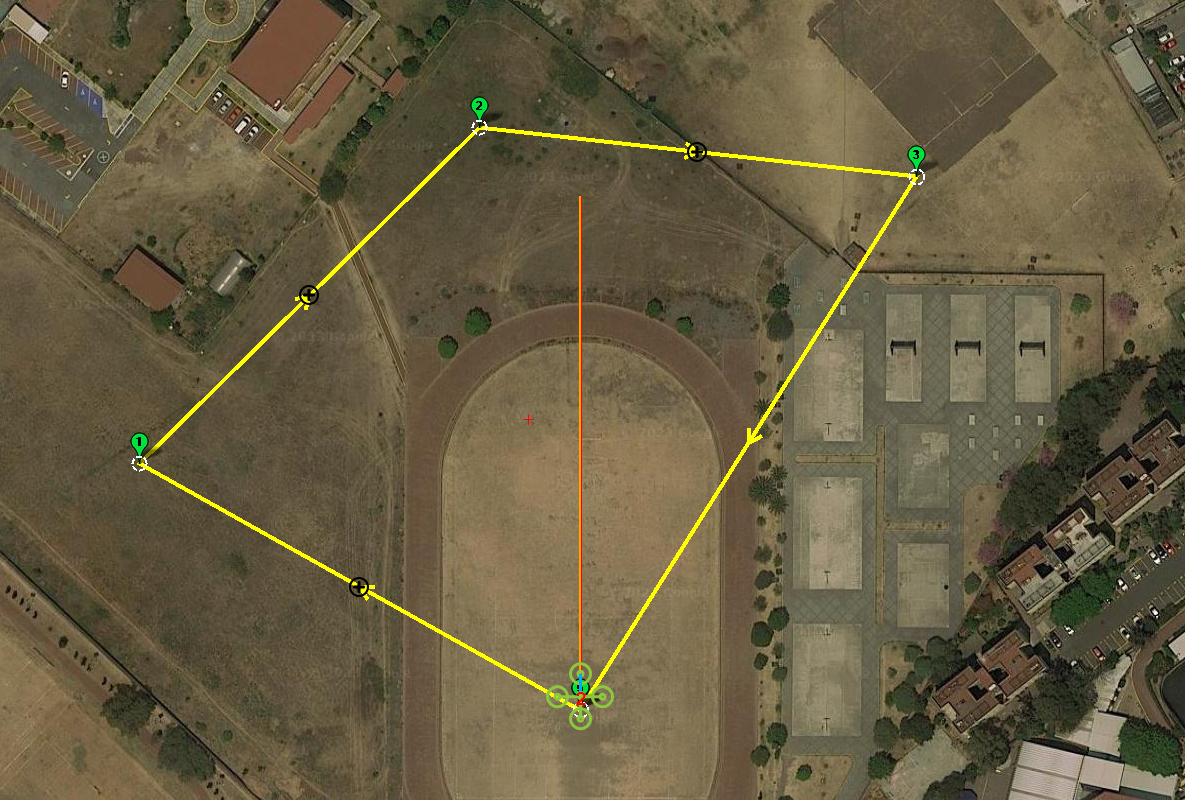
\includegraphics[width=0.7\linewidth]{imagenes/prueba_vuelo.png}
    \caption{Misión de vuelo en el campo de UPIITA-UPIBI}
    \label{fig:mision-vuelo}
\end{figure}
\newpage
Con las características mostradas en la figura \ref{fig:Características-vuelo}:
\begin{figure}[h]
    \centering
    \includegraphics[width=\linewidth]{imagenes/características.png}
    \caption{Características de la misión de vuelo.}
    \label{fig:Características-vuelo}
\end{figure}
\newpage
Para todos tenemos una altura de 30 metros y en cada punto varía el \textquotedbl{}delay\textquotedbl{} (simulando que los drones están recibiendo la información captada), posteriormente regresan al unto \textquotedbl{}Home\textquotedbl{} y aterrizan en el mismo lugar de despegue.

Otra de las características que tiene es que vuelan a una velocidad de 14.4m/s y no es posible saber en la propia simulación cuanto es el peso de cada Dron, lo que en las pruebas reales puede variar mucho los resultados; cada Dron en la simulación cuenta con una batería de 13 Volts con corriente de 3300mAh, un módulo GPS RTK y una batería cargada al 100\% como se muestra en la figura \ref{fig:Características del Dron}:

\begin{figure}[h]
    \centering
    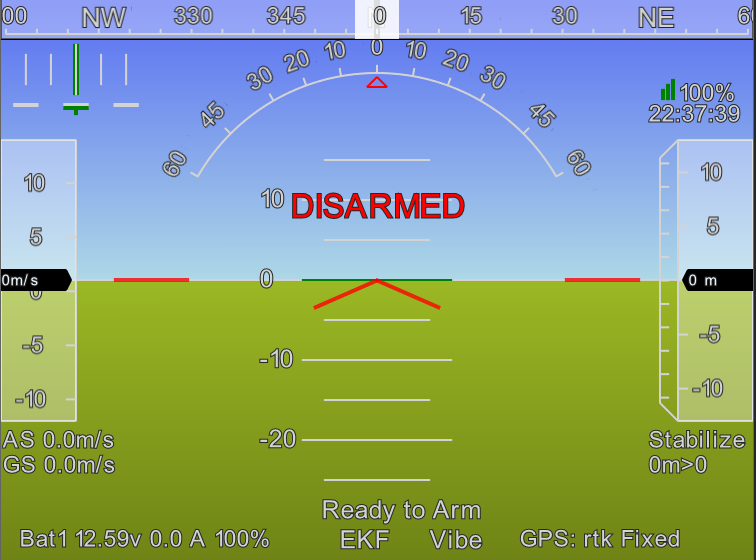
\includegraphics[width=0.8\linewidth]{imagenes/dron_caracteristicas.png}
    \caption{Pantalla de Vuelo del Dron en el Software de Mission Planner.}
    \label{fig:Características del Dron}
\end{figure}

\newpage

\subsection{Esquema de vuelo: Enjambre de Drones.}
Para esta primer simulación, haremos el esquema donde vuela el enjambre de Drones, volarán los 3 juntos y analizaremos su corriente a lo largo del trayecto.

Para los 3 drones tienen una corriente promedio de 24 A, y en completar la misión de la propuesta tardó un aproximado de 10 minutos.

Para el dron líder tenemos na corriente máxima de 32.2 A, mientras que para el Dron 2 y 3 son de 32.32 y 34.57 A. respectivamente. Sabemos que nos marca como Ampers porque en la figura \ref{fig:Características del Dron} nos muestra las unidades en Ampers.
\begin{figure}[h]

\centering
    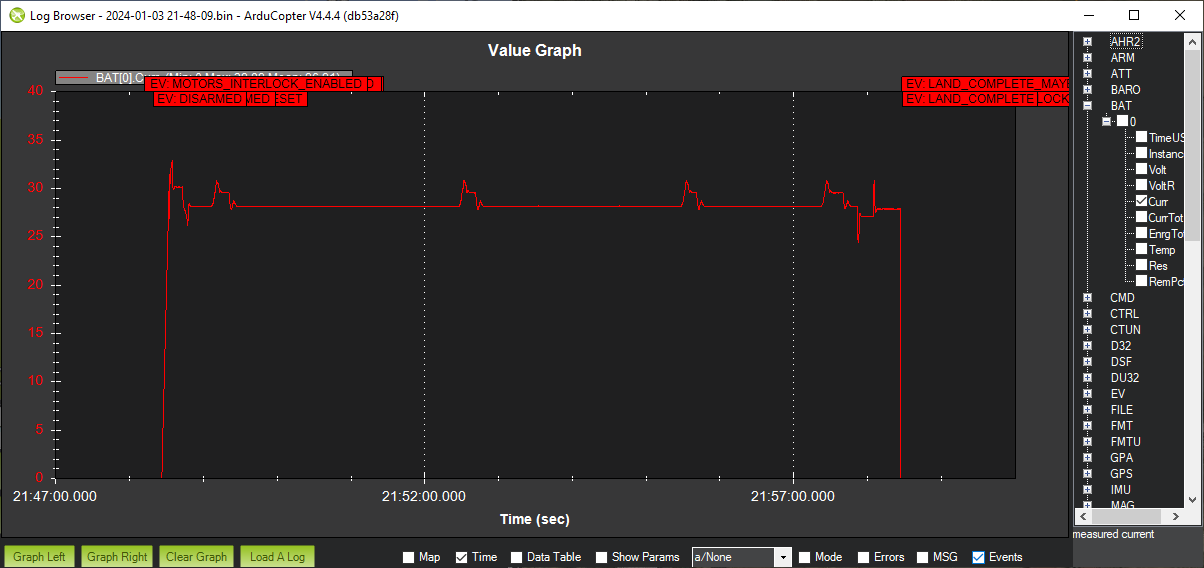
\includegraphics[width=\linewidth]{imagenes/dron_lider.png}
    \caption{Oscilograma de la corriente del dron líder.}
    \label{fig:subfig1}
\end{figure}

\newpage

\begin{figure}[h!]
    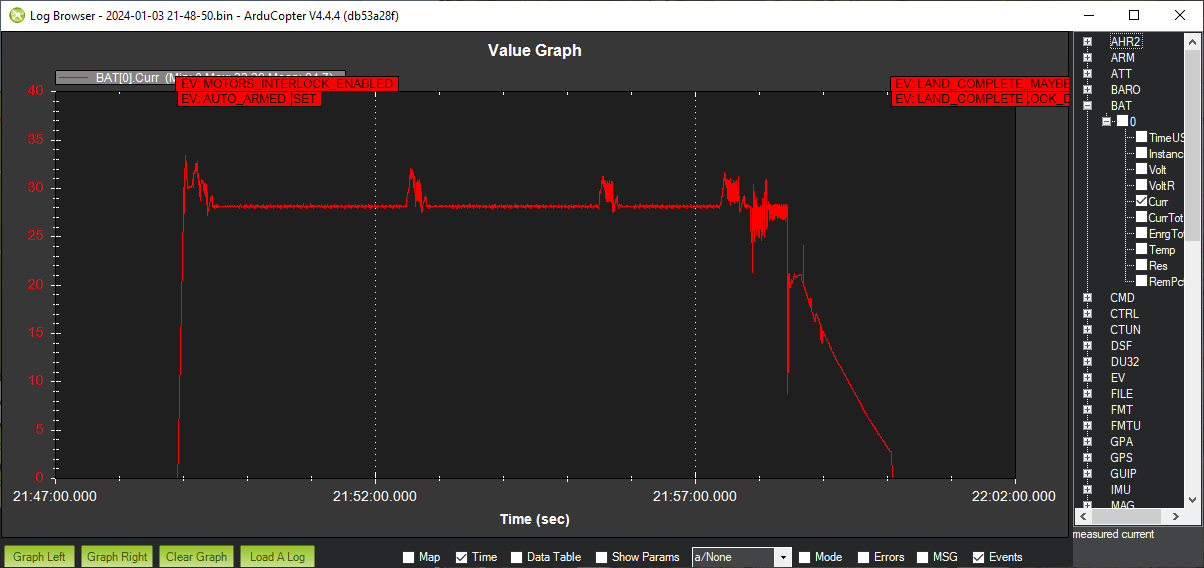
\includegraphics[width=\linewidth]{imagenes/dron_2.png}
    \caption{Oscilograma de la corriente del Dron 2.}
    \label{fig:subfig2}

    \vspace{1em} % Espacio vertical entre imágenes y leyendas

    \centering
    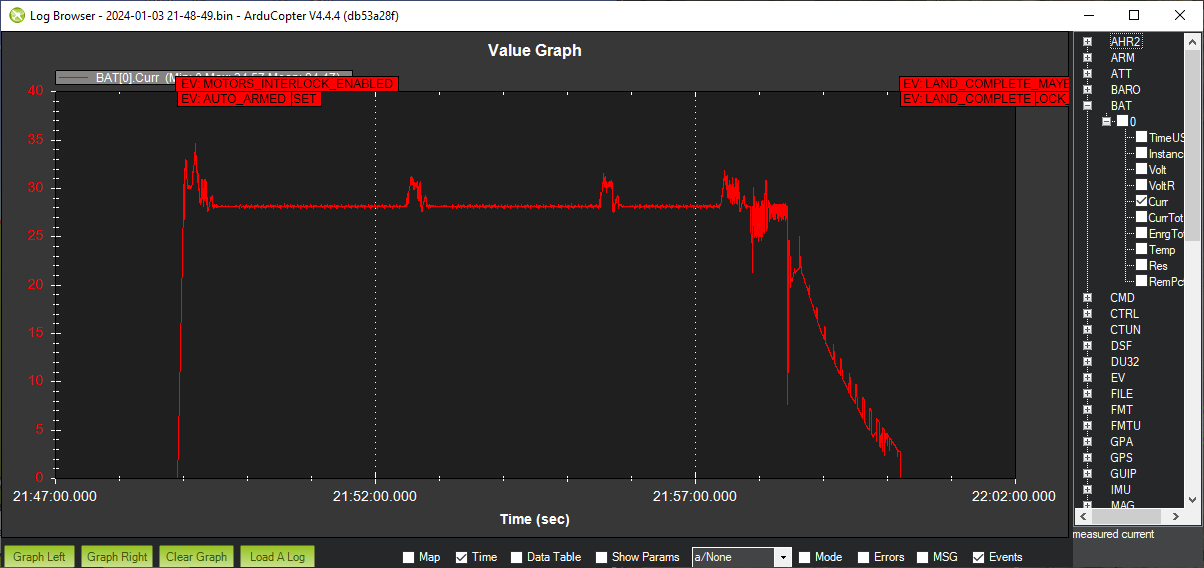
\includegraphics[width=\linewidth]{imagenes/dron_3.png}
    \caption{Oscilograma de la corriente del Dron 3.}
    \label{fig:enter-label}
\end{figure}

\newpage

\subsection{Esquema de Vuelo: Un Solo Dron.}

Para esta parte, los drones viajarán a un waypoint individualmente, los parámetros de cada vuelo se describen a continuación con sus respectivas gráficas de corriente de cada vuelo.
\begin{figure}[h!]
    \begin{minipage}{0.3\linewidth}
        \centering
        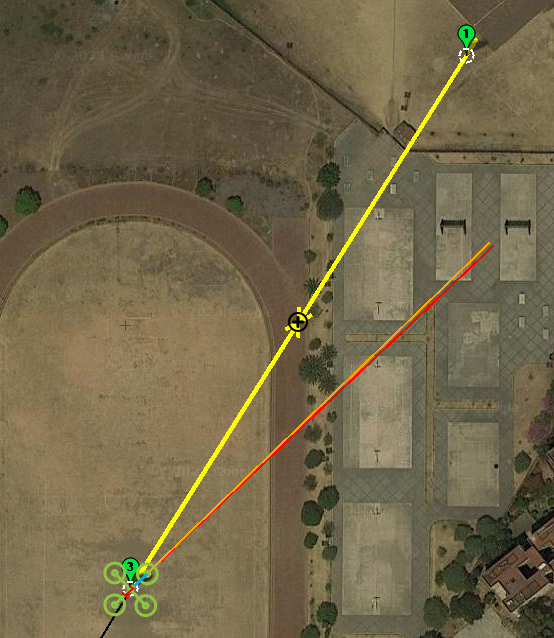
\includegraphics[width=\linewidth]{imagenes/esq_2_1.png}
        \caption{Misión de vuelo Dron 1.}
        \label{fig:subfig1}
    \end{minipage}
    \hfill
    \begin{minipage}{0.3\linewidth}
        \centering
        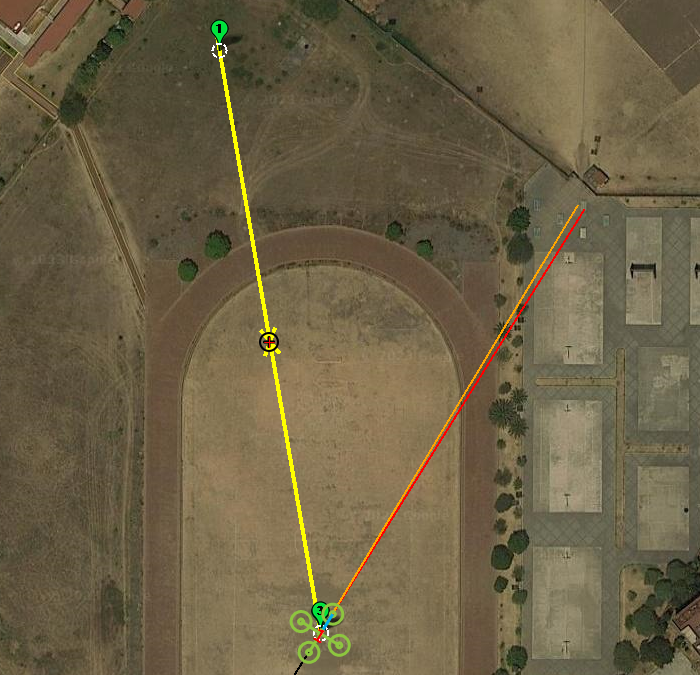
\includegraphics[width=\linewidth]{imagenes/esq_2_2.png}
        \caption{Misión de vuelo Dron 2.}
        \label{fig:subfig2}
    \end{minipage}
    \hfill
    \begin{minipage}{0.3\linewidth}
        \centering
        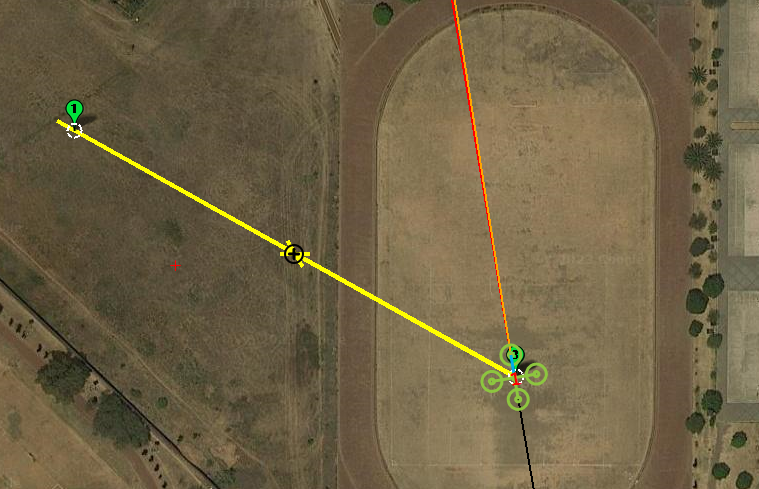
\includegraphics[width=1.1\linewidth]{imagenes/esq_2_3.png}
        \caption{Misión de vuelo Dron 3.}
        \label{fig:subfig3}
    \end{minipage}
    \caption{Misiones de vuelo de los Drones 1, 2 y 3.}
    \label{fig:enter-label}
\end{figure}

Y sus respectivas gráficas de corriente :

\begin{figure}[H]
    \centering
    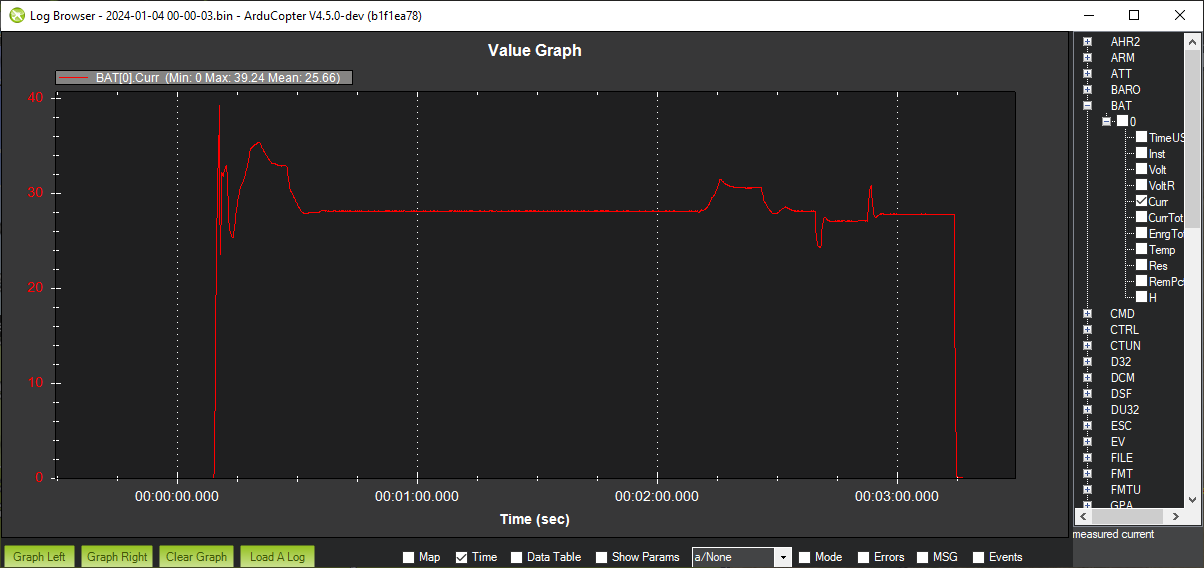
\includegraphics[width=0.9\linewidth]{imagenes/corr_2_1.png}
    \caption{Oscilograma de misión de vuelo Dron 1.}
\vspace{1cm}
 \centering
    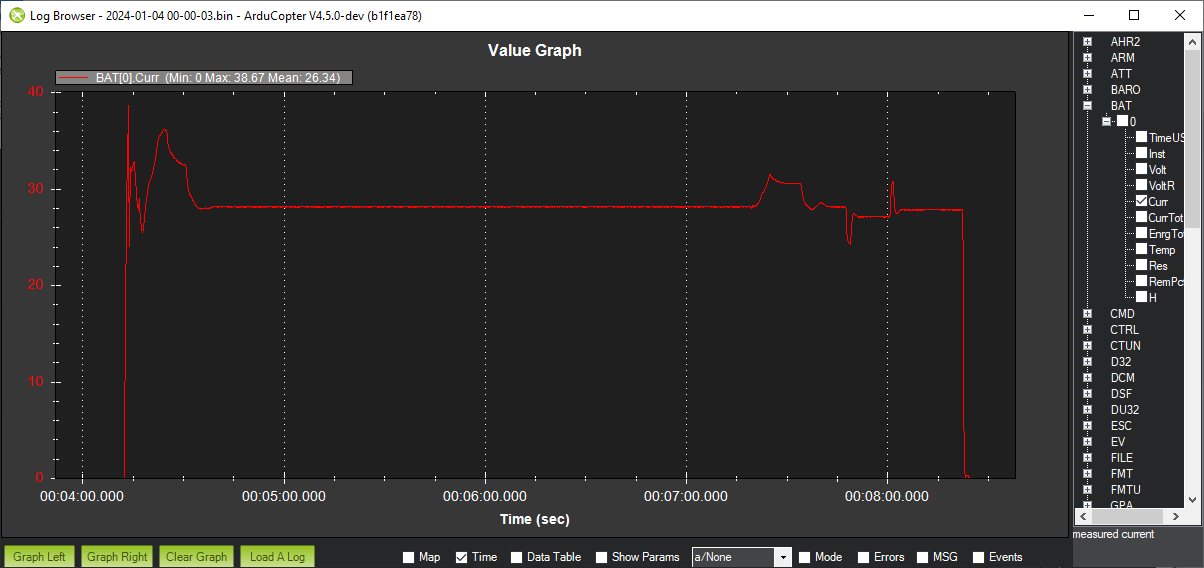
\includegraphics[width=0.9\linewidth]{imagenes/corr_2_2.png}
    \caption{Oscilograma de misión de vuelo Dron 2.}
\end{figure}
\newpage
\begin{figure}[H]    
    \centering
    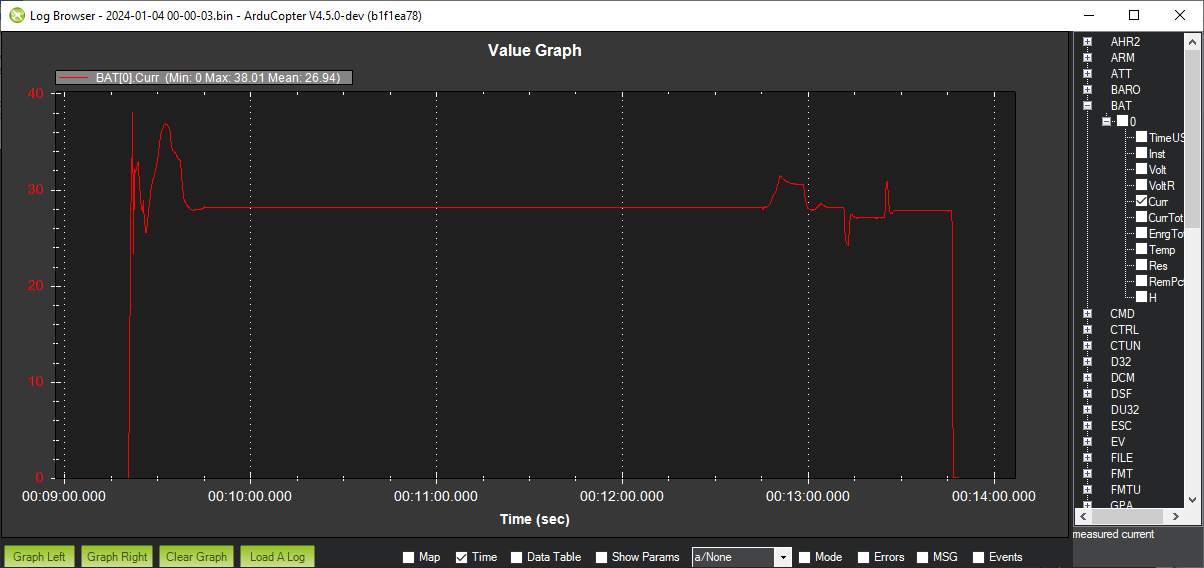
\includegraphics[width=0.9\linewidth]{imagenes/corr_2_3.png}
    \caption{Oscilograma de misión de vuelo Dron 3.}
\end{figure}

%%%%%%%%%%%%%%%%%%%%%%%%%%%%



\endinput